\documentclass{article}
\usepackage[utf8]{inputenc}
\usepackage{amsmath}

\title{Lista 6 -Aprendizado de máquina}
\author{Bruno Lucian}

\usepackage{Sweave}
\begin{document}
\Sconcordance{concordance:lista6.tex:lista6.Rnw:%
1 3 1 1 0 42 1}


\maketitle

\section*{Exercise 6.11}

\begin{itemize}
\item[(a)] O modelo nao-parametrico possui a seguinte equação para y.

\begin{equation}
g(x)=\sum\frac{\Phi(\frac{|x-x_{n}|}{\sigma})}{\sum\Phi(\frac{|x-x_{i}|}{\sigma})}y_{n}
\end{equation}
Logo, quando $|x| \to \infty$, o kernel gaussiando vai para zero fazendo o valor de $g(x) \to 0$.


O parametrico possui o seguinte comportamento,

\begin{align*}
h(x)&=\sum w_{n}z_{in}+w_{0}+\epsilon_{i} \\
&\rightarrow Y=\hat{Z}w+\epsilon \\
&\to \tilde{w}=(\tilde{Z}^{T}\overline{Z})Z^{T}y
\end{align*}

Agora quando $|x| \to \infty$, o valor da saida do kernel também vai para zero, porém, o modelo linear possui o valor de intercpeto, que não é multiplicado pela função kernel, o que faz do resultado da hipótese ser igual ao valor do intercepto.

\item[(b)] Quando $Z$ é invertível, os parâmetros da hipótese para y se descrevem da seguinte forma:

\begin{align*}
Y&=\hat{Z}w+\epsilon \\
\hat{Z}^{-1}Y&=\hat{Z}^{-1}\hat{Z}w\rightarrow w=\hat{Z}^{-1}Y
\end{align*}

Com o  $E_{in}$ 

\begin{align*}
Y-\hat{Y}&=Y-\hat{Z}\hat{Z}^{-1}Y\\ 
&\rightarrow Y-\hat{Y}=Y-IY \\ 
&\rightarrow Y-\hat{Y}=0
\end{align*}

\item[(c)] Como temos uma combinação de normais padrão temos que a esperança disso será igual a zero.  

\end{itemize}

\section*{Questão 2}

\begin{Schunk}
\begin{Sinput}
> euclid <- function(points1, points2) {
+   distanceMatrix <- matrix(NA, nrow=dim(points1)[1], ncol=dim(points2)[1])
+   for(i in 1:nrow(points2)) {
+     distanceMatrix[,i] <- sqrt(rowSums(t(t(points1)-points2[i,])^2))
+   }
+   distanceMatrix
+ }
> K_means2 <- function(x, centers, distFun) {
+   Ein<-0
+   clusterHistory <- list()
+   centerHistory <- list()
+   uni=F
+   i=1
+   while(uni==F){
+     distsToCenters <- distFun(x, centers)
+     clusters <- apply(distsToCenters, 1, which.min)
+     centers <- apply(x, 2, tapply, clusters, mean)
+     clusterHistory[[i]] <- clusters
+     centerHistory[[i]] <- centers
+     if(i > 1 && centerHistory[[i-1]]==centers){
+       uni=T
+       break
+     }
+     i=i+1
+   }
+   dados<-list()
+   erro<-list()
+   for(i in 1:nrow(centers)){
+     dados[[i]]<-x[which(clusters==i),]
+     erro[[i]]<-apply(dados[[i]],1,function(x)norm(rbind(x,centers[i,])))
+   }
+   erros<-lapply(X = erro,FUN = sum)
+   erro_geral<-sum((unlist(erros)))
+   list(clusters=clusterHistory, centers=centerHistory,erros=erro_geral)
+ }
> 
> # res <- K_means2(ktest, centers, euclid)
> 
\end{Sinput}
\end{Schunk}




\section*{Questão 3}
\begin{Schunk}
\begin{Sinput}
> require(FNN)
> data(iris)
\end{Sinput}
\end{Schunk}

\begin{Schunk}
\begin{Sinput}
> set.seed(321)
> ## Split in train + test set
> idxs <- sample(1:nrow(iris),as.integer(0.8*nrow(iris)))
> trainIris <- iris[idxs,]
> y_train <- trainIris$Species
> trainIris <- trainIris[,-5]
> testIris <- iris[-idxs,]
> y_test <- testIris$Species
> testIris <- testIris[,-5]
\end{Sinput}
\end{Schunk}

\begin{Schunk}
\begin{Sinput}
> ## A k-nn escolhendo o melhor k
> nn1 <- as.vector(as.array(knn.cv(train = trainIris,cl = y_train,k = 1)))
> nn3 <- as.vector(as.array(knn.cv(train = trainIris,cl = y_train,k = 3)))
> nn5 <- as.vector(as.array(knn.cv(train = trainIris,cl = y_train,k = 5)))
> nn7 <- as.vector(as.array(knn.cv(train = trainIris,cl = y_train,k = 7)))
> nn9 <- as.vector(as.array(knn.cv(train = trainIris,cl = y_train,k = 9)))
> nn11 <- as.vector(as.array(knn.cv(train = trainIris,cl = y_train,k = 11)))
> nn13 <- as.vector(as.array(knn.cv(train = trainIris,cl = y_train,k = 13)))
> nn15 <- as.vector(as.array(knn.cv(train = trainIris,cl = y_train,k = 15)))
> e1<-sum((nn1==y_train)==FALSE)/length(y_train)
> e3<-sum((nn3==y_train)==FALSE)/length(y_train)
> e5<-sum((nn5==y_train)==FALSE)/length(y_train)
> e7<-sum((nn7==y_train)==FALSE)/length(y_train)
> e9<-sum((nn9==y_train)==FALSE)/length(y_train)
> e11<-sum((nn11==y_train)==FALSE)/length(y_train)
> e13<-sum((nn13==y_train)==FALSE)/length(y_train)
> e15<-sum((nn15==y_train)==FALSE)/length(y_train)
\end{Sinput}
\end{Schunk}

Pela imagem podemos ver que o menos erro de previsão é onde temos o melhor $k$.

\begin{Schunk}
\begin{Sinput}
> erros<-c(e1,e3,e5,e7,e9,e11,e13,e15)
> plot(seq(1,15,by = 2),erros,type = "b",pch=16,xlab = "k vizinhos",ylab = "Erro de previsão")
\end{Sinput}
\end{Schunk}
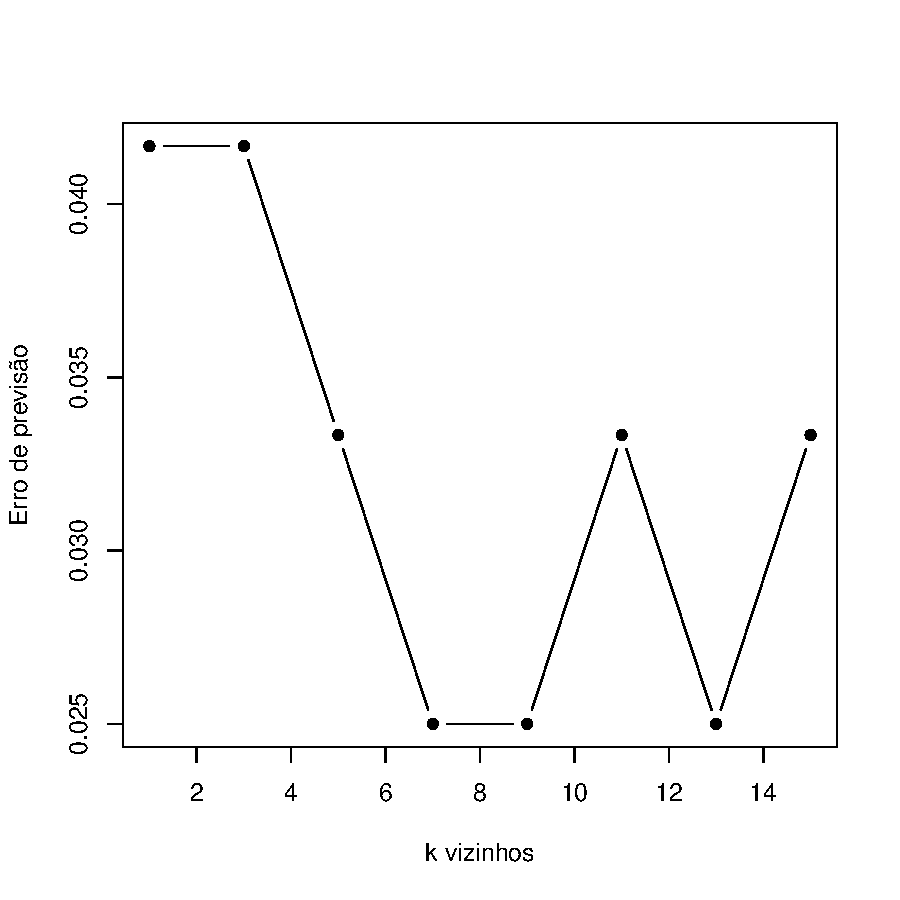
\includegraphics{lista6-005}

Escolhemos trabalhar com $k=7$ e abaixo temos a matriz de confusão.
\begin{Schunk}
\begin{Sinput}
> knn7<-as.vector(as.array(knn(train = trainIris,test = testIris,cl = y_train,k = 7)))
> table(y_test,knn7)
\end{Sinput}
\begin{Soutput}
            knn7
y_test       setosa versicolor virginica
  setosa         10          0         0
  versicolor      0          6         1
  virginica       0          0        13
\end{Soutput}
\end{Schunk}

\begin{Schunk}
\begin{Sinput}
> # load the package
> library(VGAM)
> # fit model
> fit <- vglm(Species~., family = multinomial, data=iris)
> # summarize the fit
> summary(fit)
\end{Sinput}
\begin{Soutput}
Call:
vglm(formula = Species ~ ., family = multinomial, data = iris)

Pearson residuals:
                         Min         1Q    Median        3Q       Max
log(mu[,1]/mu[,3]) -2.09e-06 -1.787e-07 4.586e-08 6.329e-08 1.327e-05
log(mu[,2]/mu[,3]) -1.97e+00 -3.382e-04 3.159e-07 4.569e-04 2.560e+00

Coefficients:
                Estimate Std. Error z value Pr(>|z|)  
(Intercept):1     34.243  42494.920   0.001   0.9994  
(Intercept):2     42.638     25.708   1.659   0.0972 .
Sepal.Length:1    10.747  12615.952   0.001   0.9993  
Sepal.Length:2     2.465      2.394   1.030   0.3032  
Sepal.Width:1     12.815   5841.307   0.002   0.9982  
Sepal.Width:2      6.681      4.480   1.491   0.1359  
Petal.Length:1   -25.043   8946.662  -0.003   0.9978  
Petal.Length:2    -9.429      4.737  -1.990   0.0465 *
Petal.Width:1    -36.060  14050.767  -0.003   0.9980  
Petal.Width:2    -18.286      9.743  -1.877   0.0605 .
---
Signif. codes:  0 ‘***’ 0.001 ‘**’ 0.01 ‘*’ 0.05 ‘.’ 0.1 ‘ ’ 1

Number of linear predictors:  2 

Names of linear predictors: log(mu[,1]/mu[,3]), log(mu[,2]/mu[,3])

Dispersion Parameter for multinomial family:   1

Residual deviance: 11.8985 on 290 degrees of freedom

Log-likelihood: -5.9493 on 290 degrees of freedom

Number of iterations: 21 
\end{Soutput}
\begin{Sinput}
> # make predictions
> probabilities <- predict(fit, iris[,1:4], type="response")
> predictions <- apply(probabilities, 1, which.max)
> predictions[which(predictions=="1")] <- levels(iris$Species)[1]
> predictions[which(predictions=="2")] <- levels(iris$Species)[2]
> predictions[which(predictions=="3")] <- levels(iris$Species)[3]
> # summarize accuracy
> table(predictions, iris$Species)
\end{Sinput}
\begin{Soutput}
predictions  setosa versicolor virginica
  setosa         50          0         0
  versicolor      0         49         1
  virginica       0          1        49
\end{Soutput}
\end{Schunk}

clustering
\begin{Schunk}
\begin{Sinput}
> require(stats)
> kmedia<-kmeans(x = iris[,-5],centers = 3,iter.max = 100)
> clusters<-kmedia$cluster
> table(clusters,iris[,5])
\end{Sinput}
\begin{Soutput}
clusters setosa versicolor virginica
       1     50          0         0
       2      0          2        36
       3      0         48        14
\end{Soutput}
\end{Schunk}




\section*{Problem 6.14}

\begin{Schunk}
\begin{Sinput}
> library(FNN)
> library(unbalanced)
\end{Sinput}
\end{Schunk}

(a) Set N = 500 and randomly split your data into a training set of size N and use the remaining data as a test/validation set.

\begin{Schunk}
\begin{Sinput}
> treino_cnn <- read.csv("train.csv")
> treino_cnn$label_novo <- as.numeric(treino_cnn$label == 1)
> treino_cnn2 <- treino_cnn[500:1000,]
> teste_cnn2 <- treino_cnn[-(500:1000),]
\end{Sinput}
\end{Schunk}


(b) Use the 3-NN algorithm with all the training data and evaluate its per- formance: report Ein and Etes.

\begin{Schunk}
\begin{Sinput}
> knn_ex4 <- (0:1)[knn(train = treino_cnn2[,-c(1,dim(treino_cnn2)[2])], test = teste_cnn2[,-c(1,dim(treino_cnn2)[2])],cl = treino_cnn2$label_novo, k = 3)]
> E_teste <- sum(knn_ex4 != teste_cnn2$label_novo)/length(teste_cnn2$label_novo)
> knn_cv_treino <- (0:1)[knn.cv(train = treino_cnn2[,-c(1,dim(treino_cnn2)[2])],cl = treino_cnn2$label_novo, k = 3)]
> E_in <- sum(knn_cv_treino != treino_cnn2$label_novo)/length(treino_cnn2$label_novo)
\end{Sinput}
\end{Schunk}

(c) Use the CNN algorithm to condense the data. Evaluate the performance of the 3-NN rule with the condensed data: report Ein and Eout.
\begin{Schunk}
\begin{Sinput}
> cnn_ex4 <- ubCNN(X = treino_cnn2[,-c(1,dim(treino_cnn2)[2])],Y = treino_cnn2$label_novo, k = 3)
> knn_cnn_ex4 <- (0:1)[knn(train = cnn_ex4$X, test = teste_cnn2[,-c(1,dim(treino_cnn2)[2])], cl = cnn_ex4$Y, k = 3)]
> E_cnn_teste <- sum(knn_cnn_ex4 != teste_cnn2$label_novo)/length(teste_cnn2$label_novo)
> knn_cnn_cv_treino <- (0:1)[knn.cv(train = cnn_ex4$X,cl = cnn_ex4$Y, k = 3)]
> E_cnn_in <- sum(knn_cnn_cv_treino != cnn_ex4$Y)/length(cnn_ex4$Y)
\end{Sinput}
\end{Schunk}

(d) Repeat parts (b) and (c) using 1000 random training-test splits and report the average Ein and Eout for the full versus the condensed data.

\begin{Schunk}
\begin{Sinput}
> E_teste_parteb <- c()
> E_in_parteb <- c()
> E_teste_partec <- c()
> E_in_partec <- c()
> for(i in 1:10)
+ {
+ 
+ treino_cnn2 <- treino_cnn[sample(1:(dim(treino_cnn)[1]),size = 500),]
+ teste_cnn2 <- treino_cnn[sample(1:(dim(treino_cnn)[1]),size = (dim(treino_cnn)[1]) - 500),]
+ 
+ #Parte (b)
+ 
+ knn_ex4 <- (0:1)[knn(train = treino_cnn2[,-c(1,dim(treino_cnn2)[2])], test = teste_cnn2[,-c(1,dim(treino_cnn2)[2])],cl = treino_cnn2$label_novo, k = 3)]
+ E_teste <- sum(knn_ex4 != teste_cnn2$label_novo)/length(teste_cnn2$label_novo)
+ knn_cv_treino <- (0:1)[knn.cv(train = treino_cnn2[,-c(1,dim(treino_cnn2)[2])],cl = treino_cnn2$label_novo, k = 3)]
+ E_in <- sum(knn_cv_treino != treino_cnn2$label_novo)/length(treino_cnn2$label_novo)
+ 
+ E_teste_parteb[1 + length(E_teste_parteb)] <- E_teste
+ E_in_parteb[1 + length(E_in_parteb)] <- E_in
+ #Parte (c)
+ 
+ cnn_ex4 <- ubCNN(X = treino_cnn2[,-c(1,dim(treino_cnn2)[2])],Y = treino_cnn2$label_novo, k = 3)
+ knn_cnn_ex4 <- (0:1)[knn(train = cnn_ex4$X, test = teste_cnn2[,-c(1,dim(treino_cnn2)[2])], cl = cnn_ex4$Y, k = 3)]
+ E_cnn_teste <- sum(knn_cnn_ex4 != teste_cnn2$label_novo)/length(teste_cnn2$label_novo)
+ knn_cnn_cv_treino <- (0:1)[knn.cv(train = cnn_ex4$X,cl = cnn_ex4$Y, k = 3)]
+ E_cnn_in <- sum(knn_cnn_cv_treino != cnn_ex4$Y)/length(cnn_ex4$Y)
+ 
+ E_teste_partec[1 + length(E_teste_partec)] <- E_cnn_teste
+ E_in_partec[1 + length(E_in_partec)] <- E_cnn_in
+ }
> mean(E_teste_parteb)
\end{Sinput}
\begin{Soutput}
[1] 0.03196386
\end{Soutput}
\begin{Sinput}
> mean(E_in_parteb)
\end{Sinput}
\begin{Soutput}
[1] 0.0326
\end{Soutput}
\begin{Sinput}
> mean(E_teste_partec)
\end{Sinput}
\begin{Soutput}
[1] 0.03193494
\end{Soutput}
\begin{Sinput}
> mean(E_in_partec)
\end{Sinput}
\begin{Soutput}
[1] 0.03253493
\end{Soutput}
\end{Schunk}


\end{document}
